\section{Validating the Neural Density Estimator} \label{sec:valid}
Our posterior (Eq.~\ref{eq:posterior}) requires an accurate estimate of the
individual posterior from NDE: 
$p(\Omega, \mathcal{B}\given {\bfi X_i}) \approx q_\phi(\Omega, \mathcal{B}\given {\bfi X_i})$
(Sec.~\ref{sec:anpe}). 
To validate $q_\phi$, we use 10\% of the CAMELS-TNG data reserved for testing
and two validation methods: (1) Simulation-Based Calibration (SBC) and (2)
the ``distance to random point'' (DRP) coverage test. 

\begin{figure}[ht]
\vskip 0.2in
\begin{center}
    \centerline{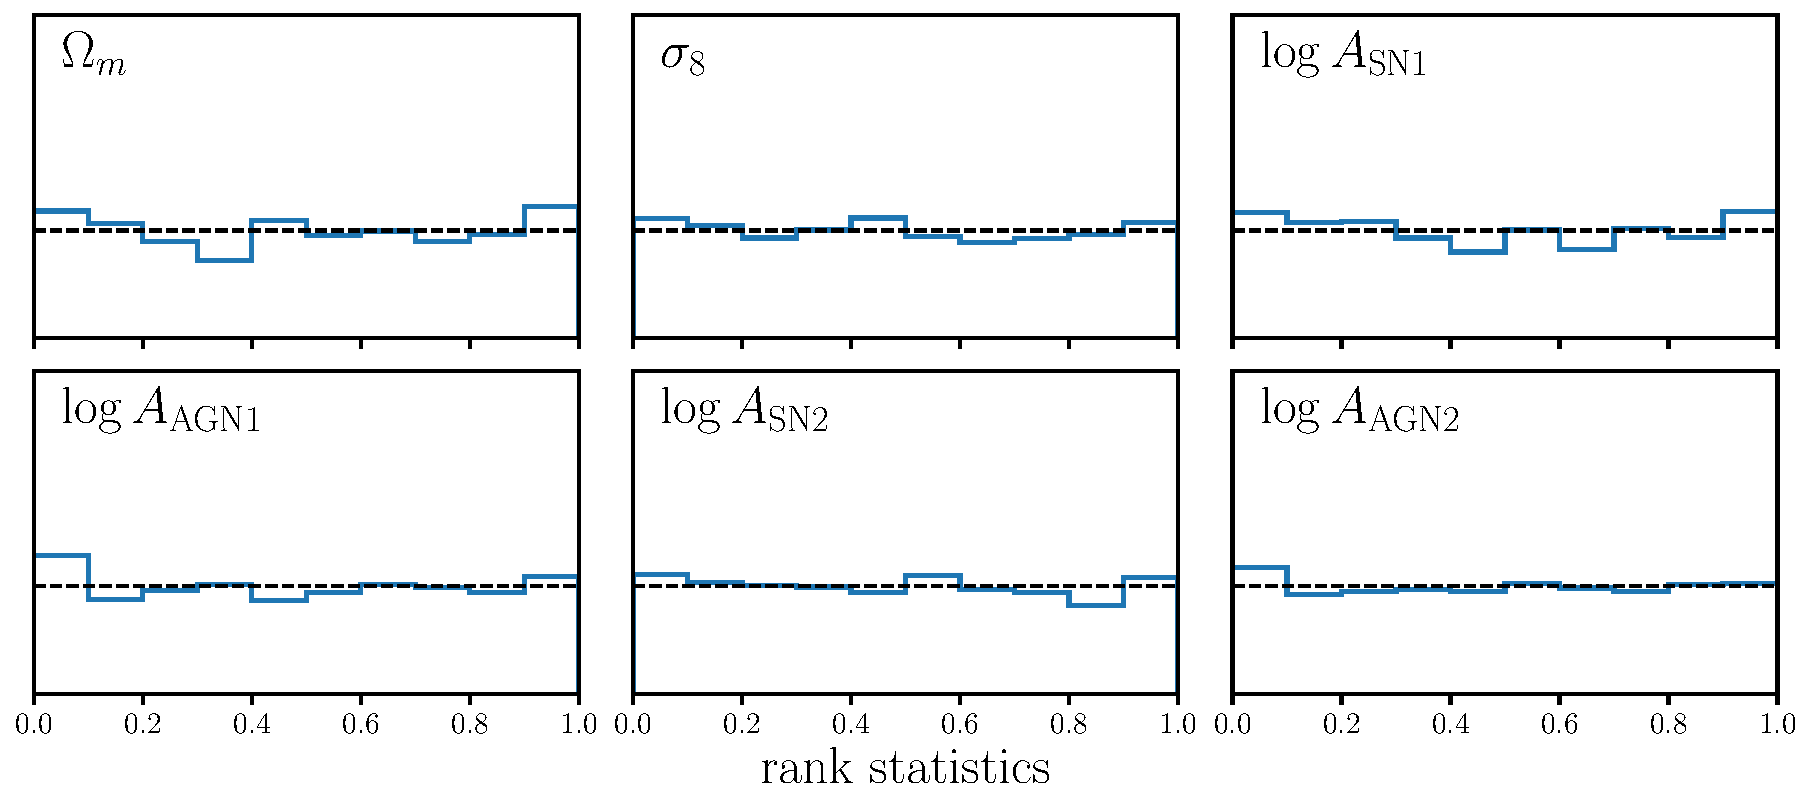
\includegraphics[width=0.9\columnwidth]{figs/ranks_p_omega_x.pdf}}
    \caption{
        Simulation-based calibration plot of 
        $q_\phi(\Omega, \mathcal{B}\given {\bfi X_i})$ using 10\% of the
        CAMELS-TNG data reserved for testing.
        The histogram in each panel represents the distribution of the rank
        statistic of the true value within the marginalized posterior (blue)
        for each parameter. 
        The rank distribution is uniform for the true posterior (black dashed).
        The rank distribution of $q_\phi$ is nearly uniform for all $\Omega$
        and $\mathcal{B}$ 
        parameters. 
        Therefore, it provides unbiased and accurate estimate of the true
        posterior.
    }\label{fig:ranks}
\end{center}
\vskip -0.2in
\end{figure}

Both are variations of the standard coverage test, where $q_\phi$ is applied to
test samples not used for training. 
The posterior of each test sample is compared against the true parameter value
its percentile score is calculated.
Afterwards, cummulative distribution function (CDF) of the percentile is used
to access the accuracy of $q_\phi$.
SBC is a modification of this standard coverage test that uses rank statistics
rather than percentile score. 
It addresses the limitation that the CDFs only asymptotically approach the true
values and that the discrete sampling of the posterior can cause artifacts in
the CDFs. 
In Fig.~\ref{fig:ranks}, we present the SBC rank distributions of $q_\phi$ for
$\Omega$ and $\mathcal{B}$ (blue). 
For the true posterior, rank distribution is uniform by construction (black
dashed).
The rank distributions are nearly uniform for all $\Omega$ and
$\mathcal{B}$.
Hence, we confirm that $q_\phi$ is in excellent agreement with the true
posterior.


\begin{figure}[ht]
\vskip 0.2in
\begin{center}
    \centerline{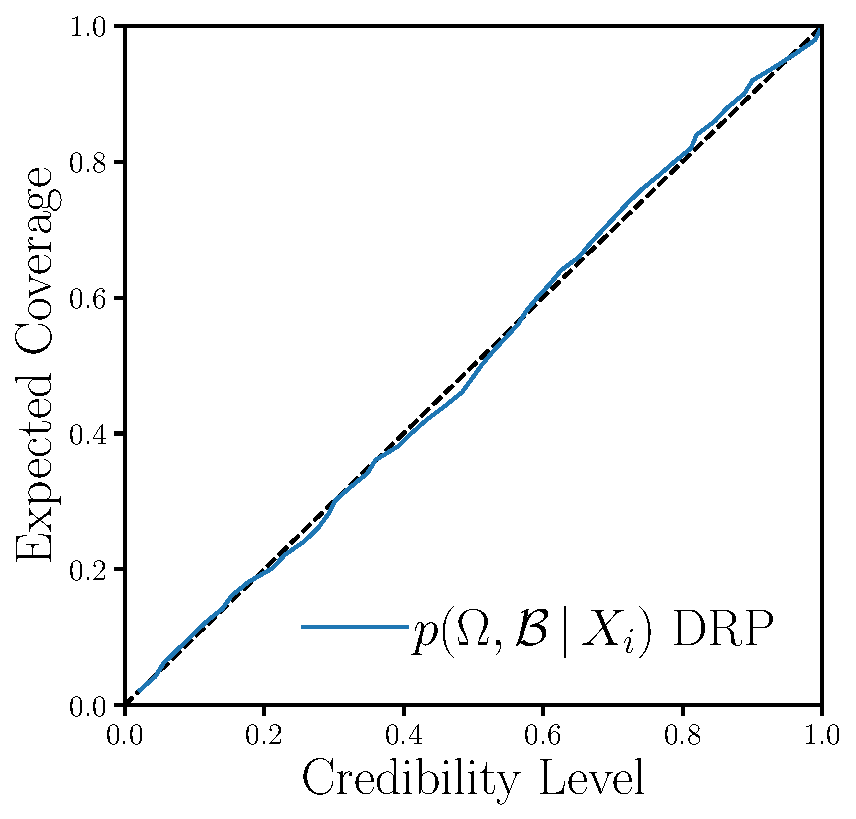
\includegraphics[width=0.4\columnwidth]{figs/tarp_p_omega_x.pdf}}
    \caption{DRP coverage test validating the accuracy of our 
    $q_{\phi}(\Omega, \mathcal{B}\given {\bfi X_i})$ posterior estimate (blue).
    The DRP test is calculated using  10\% of the CAMELS-TNG data reserved for
    testing.
    The black-dashed line represents an optimal estimate of the posterior.
    The DRP test demonstrates that $q_\phi$ provides a near optimal
    estimate of the true posterior.
    }\label{fig:tarp}
\end{center}
\vskip -0.2in
\end{figure}

As additional validation, we also use the DRP coverage test from
\cite{lemos2023}.
Instead of percentile scores or ranks, the DRP test assesses $q_\phi$ using
samples drawn from $q_\phi$ for a test sample, the true parameter value of the
test sample, and a random point in parameter space. 
It evalulates the distances between the $q_\phi$ samples and the random point. 
Then compares the distances to the distance between the true parameter value
and the random point in order to derive an estimate of expected coverage
probability. 
\cite{lemos2023} prove that this approach is necessary and sufficient to show
that a posterior estimator is optimal.
In Fig.~\ref{fig:tarp}, we present the DRP coverage test of $q_\phi$ (blue). 
Based ont he DRP test, $q_\phi$ provides a near optimal estimate of the
true posterior (black-dashed). 

